\documentclass[12pt, twoside]{article}
\usepackage{jmlda}
\usepackage{bm}
\usepackage{amsmath}
\newcommand{\hdir}{.}

\begin{document}
\English

\title
	[] % short title for page headings, not necessary if a full title fits the headings
    {Additively Regularized Multimodal Topic Hierarchies} % full title
\author
	[] % short list of the authors (<= 3) for page headings, is necessary only if the full list does not fit the headings
	{N.\,A.~Chirkova, K.\,V.~Vorontsov} % full list of the authors, presented in the table of contetns of the issue
    [N.\,A.~Chirkova$^1$, K.\,V.~Vorontsov$^2$] % list of the authors presented in the title page of the article, is necessary only if it differs from the full list of the authors in braces, i.e. '{' and '}'
\email
    {nadiinchi@gmail.com, vokov@forecsys.ru}
\thanks
    {}
\organization
    {$^1$Lomonosov Moscow State University, Leninskie Gory, 1, Moscow, Russia;
     $^2$ORGANIZATION}
\abstract
    {AAA ``Machine Learning and Data Analysis''.
		
	\noindent
	BBB


	
	\noindent
	\textbf{Background}:	One paragraph about the problem, existent approaches and its limitations.
	
	\noindent
	\textbf{Methods}: One paragraph about proposed method and its novelty.
	
	\noindent
	\textbf{Results}: One paragraph about major properties of the proposed method and experiment results if applicable.
	
	\noindent
	\textbf{Concluding Remarks}: One paragraph about the place of the proposed method among existent approaches.
		
	\noindent
    	\textbf{Keywords}: \emph{topic modeling; ARTM; topic hierarchies; regularization}}

\titleRus
    [] % short title for page headings, not necessary if a full title fits the headings
    {Аддитивно регуляризованные многомодальные тематические иерархии} % full title
\authorRus
    [] % short list of the authors (<= 3) for page headings, is necessary only if the full list does not fit the headings
    {Н.\,А.~Чиркова, К.\,В.~Воронцов} % full list of the authors, presented in the table of contetns of the issue
    [Н.\,А.~Чиркова$^1$, К.\,В.~Воронцов$^2$] % list of the authors presented in the title page of the article, is necessary only if it differs from the full list of the authors in braces, i.e. '{' and '}'
\thanksRus
    {}
\organizationRus
    {$^1$Московский государственный университет им. М.\,В.\,Ломоносова $^2$Организация}
\abstractRus
    {
	
\bigskip
\noindent
\textbf{Ключевые слова}: \emph {тематическое моделирование; АРТМ;  тематические иерархии; регуляризация}
}


%these fields are filled in by the journal editors
\doi{10.21469/22233792}
\receivedRus{12.05.2016}
\receivedEng{May 12, 2016}

\maketitle
\linenumbers

\newcommand{\norm}{\mathop{\text{norm}}}

\section{Introduction}
\noindent %this command is placed at the beginning of the first sentence of each paragraph/section only.
Multiple inheritance:

It is common case in any field of knowledge when specific topic occurs on the edge of two or even more major topics. For example, bioinformatics combines applied mathematics and computer science to solve biology problems. 

Feature: multiple inheritance \& ability to make graph sparse

Feature: fast

Feature: combination with other regularizers

\section{Related Work}
Briefly: PLSA, LDA, ARTM. These are plate models/

hierarchical approaches

hvHDP: bottom up, child topic as documents

STROD: parent topic distribution is a mixture of child topic distributions



\section{Problem statement}
In this paper we refer to the document collection as $D$ consisting of documents of different subjects.
Documents may contain not only words but other elements too, say tags, links, location marks etc. We refer to such types of elements as modalities. For example, scientific paper can be described at least by three modalities: text, keywords and references. $M$ denotes a set of all modalities in the collection. Modalities $m \in M$ are defined by disjoint dictionaries $W = \bigsqcup_{m \in M} W^m$. 

A document $d \in D$ is a sequence of $n_d$ elements: $(w_1, w_2, w_3, \dots)$, $w_i \in W$. In this paper an order of elements is not important. Thus collection can be represented as a counters matrix $\{n_{dw}\}_{D \times W}$, $n_{dw}$ is a number of $w$ occurencies in $d$.

Given the text collection, our goal is to organize its documents into comprehensive hierarchical structure. We define \emph{topic hierarchy} as an oriented multipartitle (multilevel) graph of topics so that edges connect topics from neighboring levels. If there is an edge $a \rightarrow t$ in hierarchy then topic $a$ is called \emph{parent}, or \emph{ancestor} topic and $t$ is called \emph{child topic}, or \emph{subtopic}. Parent topic is divided into several more specific child topics. 
Obviously, number of topics on each following (child) level must be greater than on previous (parent) level. Zero level consists of only one topic called \emph{root}. AN example of topic hierarchy is given on pic.~\ref{fg:hierarchy}.

Each topic in hierarchy is associated with distributions over each modality dictionary. This allows us to represent a topic by a top of most probable words saying what this topic is about. The same can be done with other modalities.
\begin{figure}[!th]
	\begin{center}
		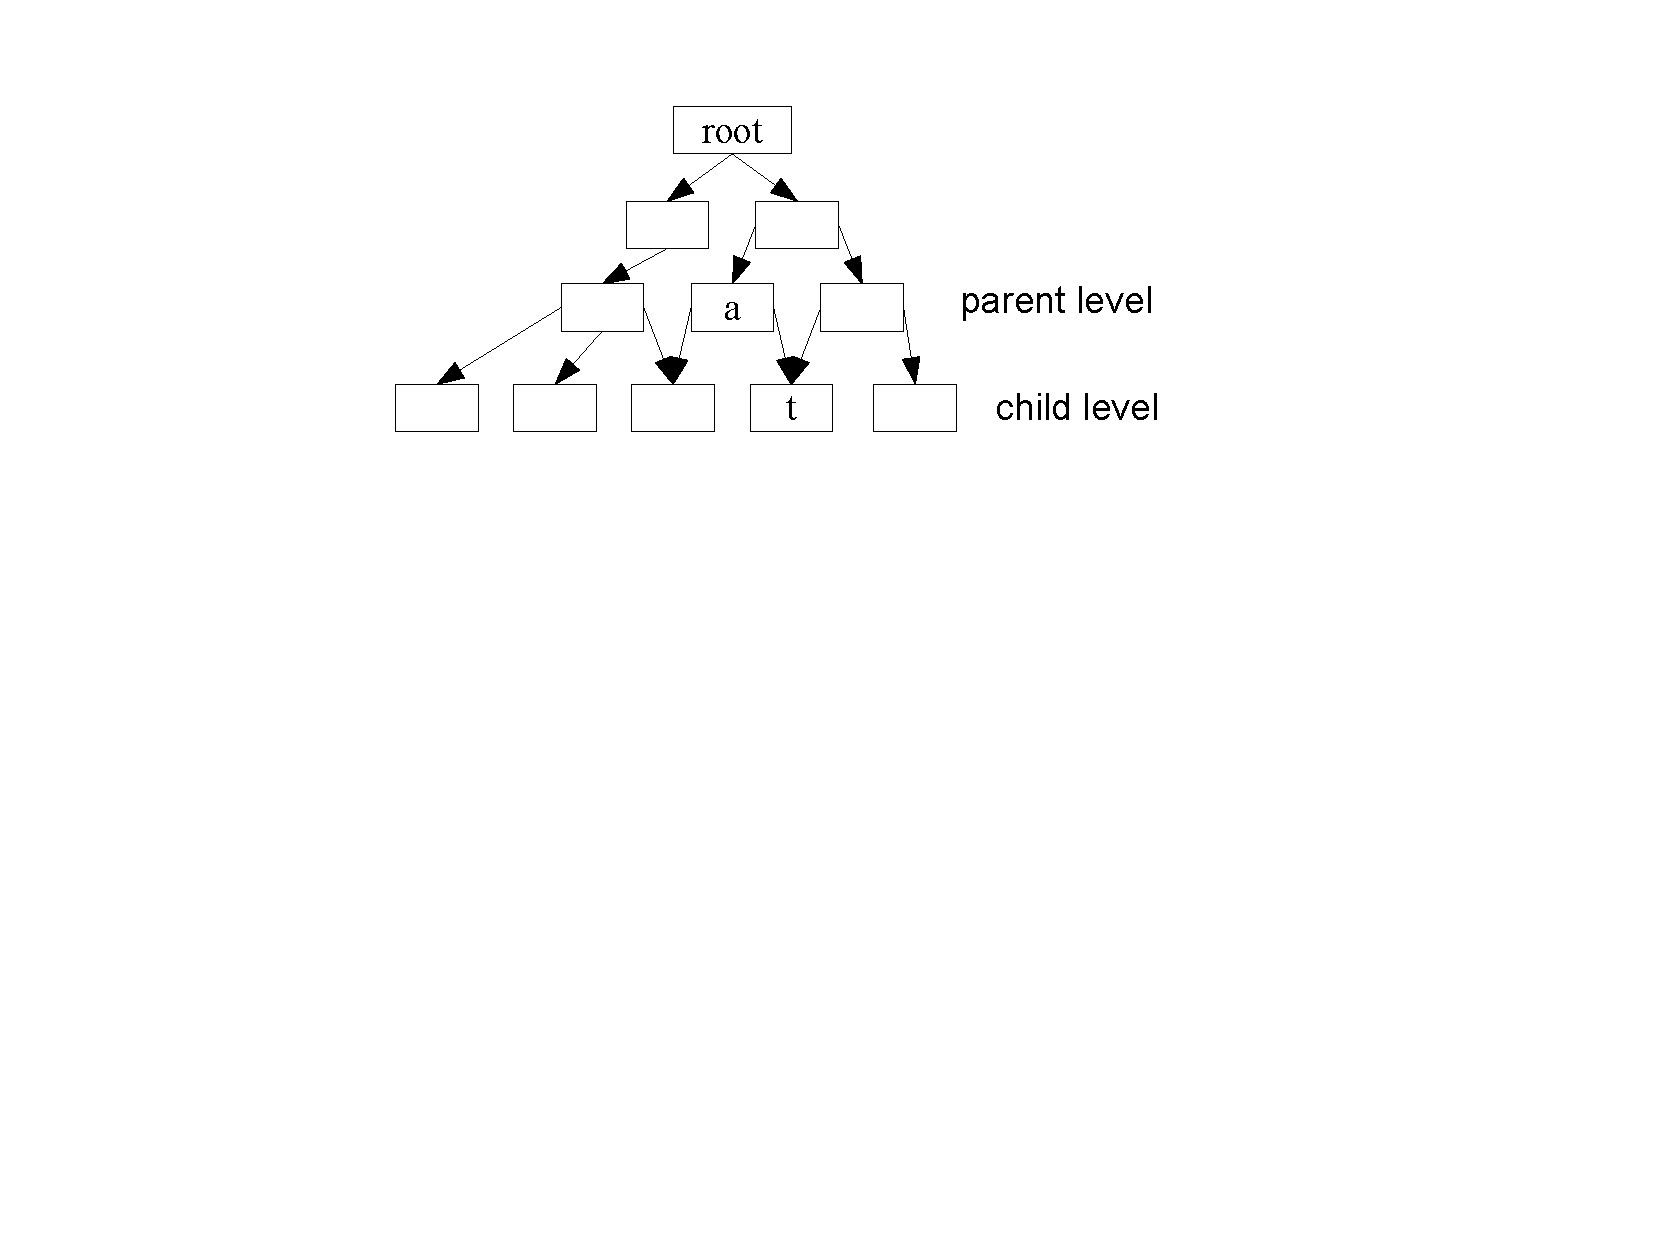
\includegraphics[width=0.4\linewidth]{\hdir/hierarchy_definition.pdf}
	\end{center}
	\caption{An example topic hierarchy}
	\label{fg:hierarchy}
\end{figure}

To learn hierarchy we combine several plate topic models and tie them via regularization.

In the rest of the paper we will use operator 
$\norm\limits_{x \in X} [y_x] = \frac{( y_x )_+}
{\sum_{x' \in X}( y_{x'})_+}$ transforming real vector to probability distribution, $(y_x)_+$ equals $y_x$ if $y_x > 0$ and $0$ otherwise.


%In such formulation each topic except root may have more than one parent topics. 

\section{hARTM framework}
\subsection{ARTM: plate topic models}
Plate topic model describes collection $D$ by finite topics set $T$. In ARTM~\cite{ARTM} document distribution over each modality is modeled as a mixture of topics distributions:
\[
p(w|d) \approx \sum_{t \in T} p(w|t) p(t|d)   \quad  d \in D, \, w \in W^m.
\]
In other words, for each modality $m$ topic model is a low-rank approximation 
\[
F^m\approx \Phi^m \Theta
\]
of frequency matrix $F^m = \{f_{wd}\}_{W^m \times D}$, $f_{wd} = \norm\limits_{w \in W^m} [n_{dw}]$ estimating $p(w|d)$ with parameters $\Phi^m = \{\phi_{wt}\}_{W^m \times T}$, $\phi_{wt} = p(w|t)$ and $\Theta = \{\theta_{td}\}_{T \times D}$, $\theta_{td} = p(t|d)$. $\Phi$ and $\Theta$ are stochastic matrices:
\begin{equation}
	\label{constrains}
\sum_{w \in W^m} \phi_{wt} = 1, \quad \sum_{t \in T} \theta_{td} = 1.
\end{equation}
For brevity we denote vertically stacked $\Phi^m$, $m \in M$ and $F^m$, $m \in M$ by $\Phi$ and $F$ respectively. Then topic model in approximate matrix factorization $F \approx \Phi \Theta$.
% Parameters $\Theta$ specify the proportions of topics in documents, or weights of topics in the mixture.

We use regularized weighted maximum log-likelihood principle to learn $\Phi$ and $\Theta$ :
\begin{equation}
\label{optimization_problem}
    \sum_{m \in M} \kappa_m \sum_{d \in D} \sum_{w \in W^m} n_{dw} \ln \sum_{t \in T} \phi_{wt} \theta_{td} + \sum_i \tau_i R_i(\Phi, \Theta) \rightarrow \max_{\Phi, \Theta}.
\end{equation}
Weights $\kappa_m$ are used to balance log-likehood of modalities. Regularizers $R_i$ impose additional subject-specific criteria for model parameters. Regularizer coefficients $\tau_i$ balance optimization of regularizers and log-likehood. If regularizer term $R = \sum_i \tau_i R_i(\Phi, \Theta)$ equals zero and there is only text modality then described model simplifies to PLSA.

\begin{Theorem}[Vorontsov, Potapenko, 2014]
If all regularizers are continuously differentiable on $\Phi$ and $\Theta$, then the stationary point of problem \eqref{optimization_problem} with constrains \eqref{constrains} satisfies the following system yielding EM-algorithm for model training:

\begin{equation*}
	\begin{split}
	 \text{E-step}: \quad & p(t|d, w) = \norm\limits_{t \in T} [\phi_{wt} \theta_{td}], \quad w \in W, \, d \in D ;\\
	 \text{M-step}: \quad & \phi_{wt} = \norm\limits_{w \in W^m} \biggl[n_{wt} + \frac{\partial R}{\partial \phi_{wt}} \phi_{wt}\biggr], \quad n_{wt} = \sum_{d \in D} n_{dw} p(t| d, w) ;\\
	 & \theta_{td} = \norm\limits_{t \in T} \biggl[n_{td} + \frac{\partial R}{\partial \theta_{td}} \theta_{td}\biggr], \quad n_{td} = \sum_{w \in W} n_{dw} p(t| d, w).
	 \end{split}
\end{equation*}
\end{Theorem}
EM-algorithm is obtained by applying the fixed point iteration method to the system.

Hyperparameters of plate topic model are number of topics $|T|$ and weights $\{\kappa_m\}_{m \in M}$, $\{\tau_i\}_{i}$. While learning topic hierarchy, we will need to train plate topic model for each level of hierarchy, every time with new hyperparameters settings.

\subsection{hARTM: top-down hierarchy learning}
Since topic hierarchy is a multilevel graph, we consider each level as a plate topic model. Zero level is associated with the whole collection. The first level contains small number of major topics. Starting from second level, we need not only to model topics, but also to establish parent-child topic relations. To do this, we introduce two additional matrix factorization problems and propose two new interchangeable regularizers based on them. 

Assume we have already learned $\ell \geqslant 1$ hierarchy levels. Now we will learn $(\ell+1)$-th level that is child level for $\ell$-th ancestor level. Not to confuse levels we denote parent level topics $a \in A$ and parameters $\Phi^\ell$, $\Theta^\ell$ instead of $t \in T$, $\Phi$ and $\Theta$ used for child level. Note that $\Phi^\ell$ and $\Theta^\ell$ are already modeled.

\textbf{$\Phi$ regularizer.}
We suppose that parent topic distribution over words and other modalities should be a mixture of child topics distributions:
\[
p(w|a) = \sum_{t \in T} p(w|t) p(t|a), \quad w \in W^m, \, a \in A.
\] 
% Гипотеза условной независимости?
This means an approximation 
\begin{equation}
\label{phi_approximation}
\Phi^\ell \approx \Phi \Psi
\end{equation}
 with new parameters matrix $\Psi = \{\psi_{ta}\}_{T \times A}$, $\psi_{ta} = p(t|a)$ containing \emph{interlevel distributions} of children topics in parent topic. If the measure of probability distributions dissimilarity is Kullback–Leibler divergence, we have the following regularizaion criteria:
\begin{equation}
\label{phi_regularizer}
\nonumber
 \sum_{a \in A} n_a \, KL(\bm \phi^{\ell, m}_a \| \Phi^m \, \bm \psi_a)  \rightarrow \min_{\Phi^m, \Psi}
\end{equation}
or, equivalently,
\[
R(\Phi^m, \Psi) = \sum_{a \in A} \sum_{w \in W^m} n_{wa} \ln \sum_{t \in T} \phi_{wt} \psi_{ta} \rightarrow \max_{\Phi^m, \Psi},
\]
$\bm \phi^{\ell, m}_a$ and $\bm \psi_a$ denote columns of $\Phi^{\ell, m}$ and $\Psi$ respectively. Weights $n_a = \sum_{w \in W^m} n_{wa}$ are imposed to balance parent topics proportionally to their size and to scale criteria up to log-likelihood scale, $n_{wa}$ are parent topic counters from EM-algorithm.
Regularizer criterias are weighted by modalities weights: 
\[
R(\Phi, \Psi) = \sum_{m \in M} \kappa_m R(\Phi^m, \Psi).
\]

This regularizer is equivalent to adding $|A|$ pseudodocuments to collection represented by $\{n_{wa}\}_{W \times A}$ columns. Then $\Psi$ forms additional columns to $\Theta$ corresponding to pseudodocuments. Note than child level couldn't be trained only on pseudodocuments because internal dimension in approximation \eqref{phi_approximation} is higher than the minimum dimension of $\Phi^\ell$ and $\Phi$ will just copy columns of $\Phi^\ell$.

\textbf{$\Theta$ regularizer.}
The same idea may be applied for regularizing $\Theta$ instead of $\Phi$. Then for each document distribution over parent topics is a mixture of topic distributions:   % ???
\[
p(a|d) = \sum_{t \in T} p(a|t) p(t|d).
\]
Additional matrix approximation looks like
\begin{equation}
    \nonumber
    \Theta^\ell \approx \widetilde \Psi \Theta 
\end{equation}
with interlevel distributions $\widetilde \Psi = \{\tilde \psi_{at}\}_{A \times T}$, $\tilde \psi_{at} = p(a|t)$. This means that parent topic's documents set is a union of children's documents sets. Regularizer criteria:
\[
R(\Theta, \widetilde \Psi) = \sum_{a \in A} \sum_{d \in D} \theta^\ell_{ad} \ln \sum_{t \in T} \tilde \psi_{at} \theta_{td} \rightarrow \max_{\widetilde \Psi, \Theta}.
\]
To train child model with regularizer we add new modality $\tilde m$ corresponding to parent topics and consider document counters for this modality are $\theta^\ell_{ad}$. $\Theta$-regularizer coefficient will become modality weight and $\widetilde \Psi$ will correspond to $\Phi^{\tilde m}$.
\begin{figure}[!th]
	\begin{center}
	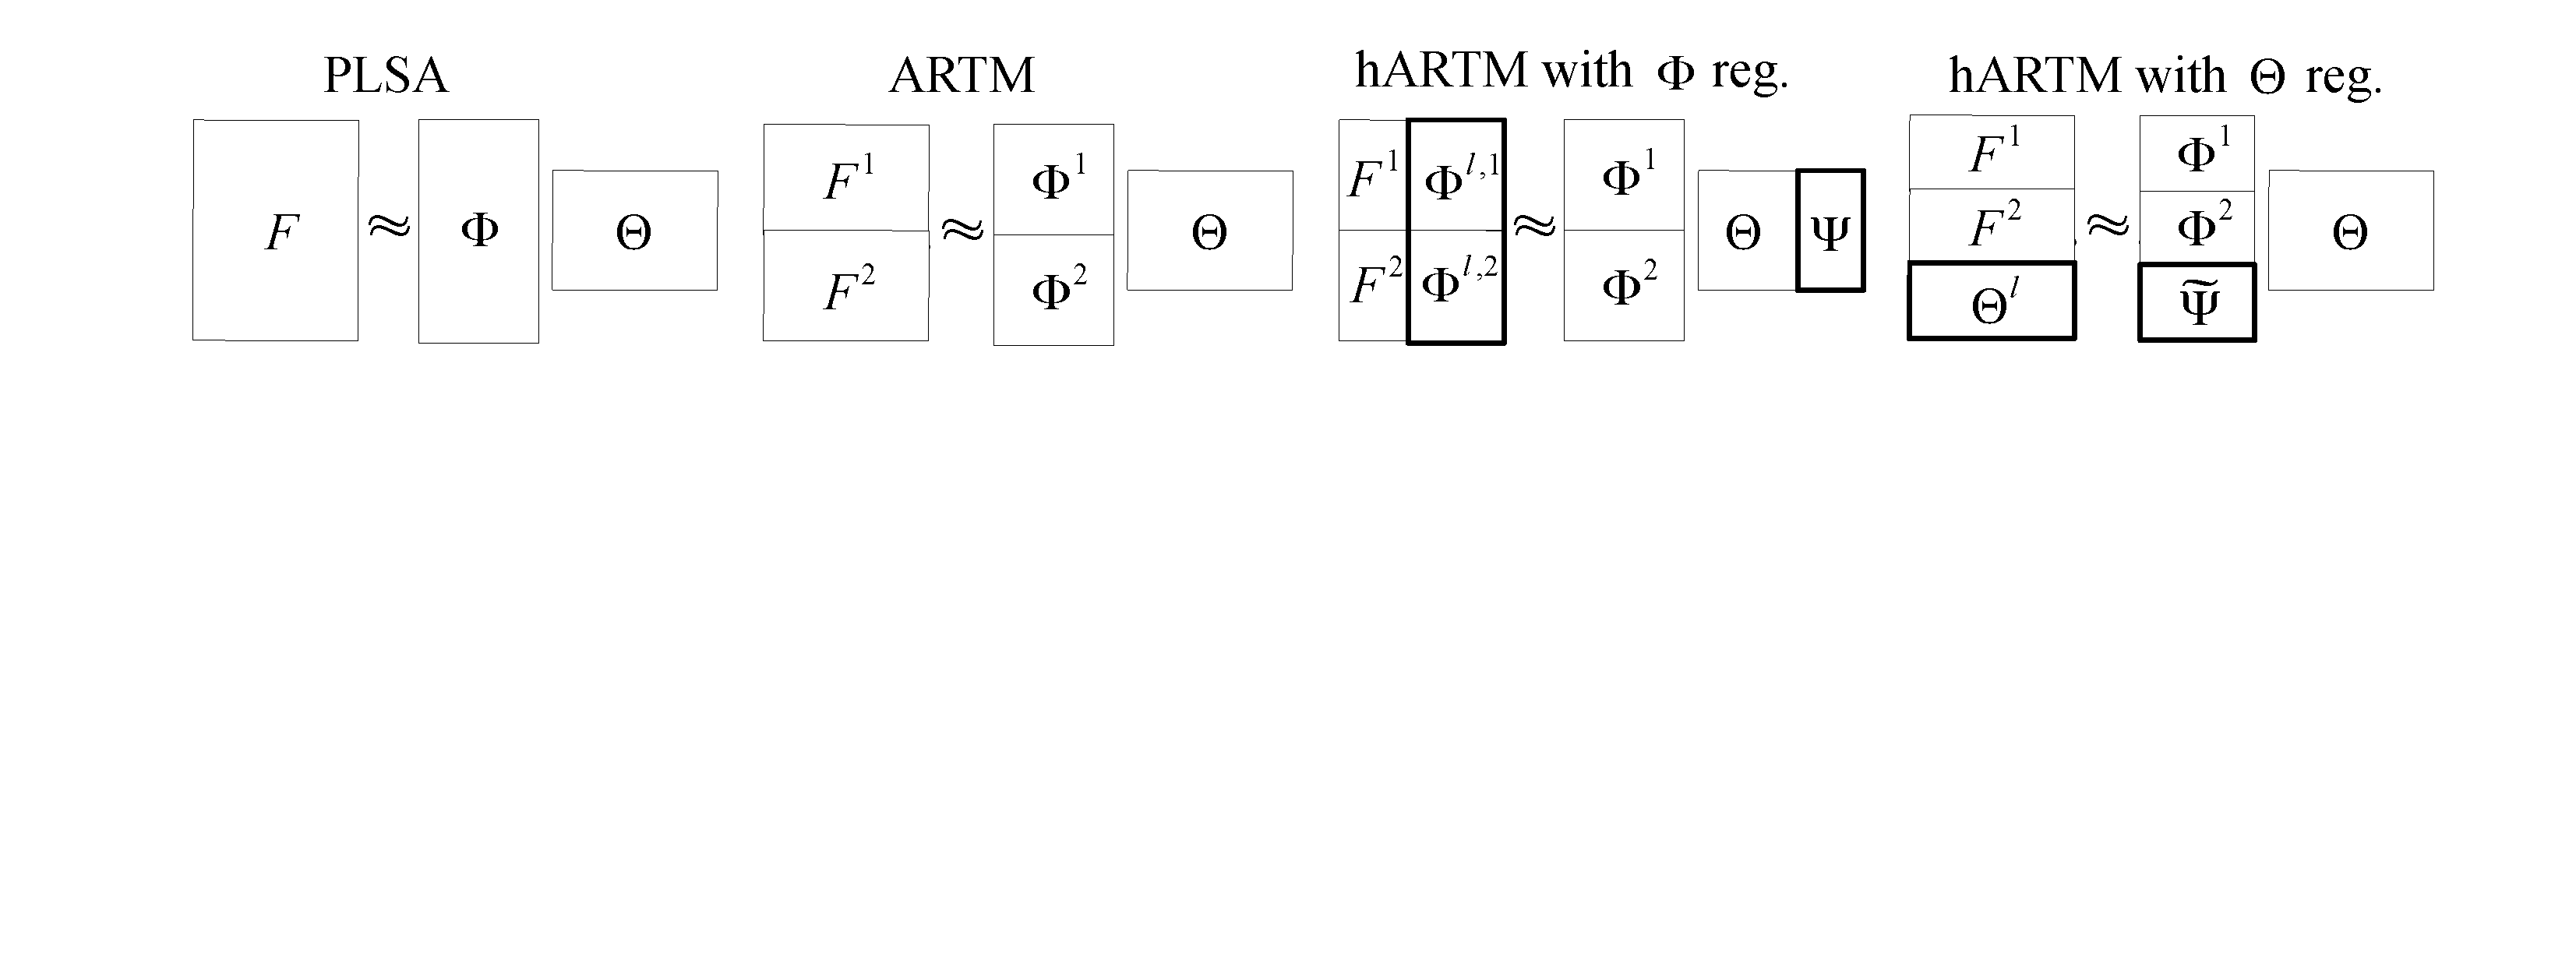
\includegraphics[width=0.55\linewidth]{\hdir/matrices_illustration.pdf}
\end{center}
\caption{An illustration of child level regularization}
\label{fg:matrices}
\end{figure}

\vspace{0.5cm}
An illustration of manipulating with pseudodocuments and new modality while the regularization of child level is given on pic.~\ref{fg:matrices}.  Note that when learning $(\ell+1)$-th level only $\ell$-th level's topics are used for regularization, not all previous levels' topics. 




%High rank, only as regularizer. Idea similar to Zavitsanos.
\subsection{Hierarchy sparsing}

\section{Implementation in BigARTM, open-source topic modeling library}

\section{Experiments}

\section{Discussion}

%%%% please specify doi of the cited item if possible, see~\bibitem{article}
%%%% Crossref doi of the item can be retrieved at http://www.crossref.org/guestquery/
\begin{thebibliography}{99}

\bibitem{book}
	\BibAuthor{Goossens,~M., F. Mittelbach, and A.~Samarin}. 1994.
	\BibTitle{The \LaTeX\ companion}.
	2nd ed.
	Reading, MA: Addison-Wesley. 528 p.

\bibitem{article}
	\BibAuthor{Zagurenko,~A.\,G., V.\,A.~Korotovskikh, A.\,A.~Kolesnikov, A.\,V.~Timonov, and D.\,V.~Kardymon}. 2008.
	Tekhniko-ekonomicheskaya optimizatsiya dizayna gidrorazryva plasta
	[Technical and economic optimization of the design of hydraulic fracturing].
	\BibJournal{Neftyanoe Khozyaystvo} [Oil Industry] 11(1):54--57.
	\BibDoi{10.3114/S187007708007}. (In Russian)

\bibitem{webArticle}
	\BibAuthor{Blaga,~P.\,A.} 2007.
	Commutative Diagrams with XY-pic II. Frames and Matrices.
	\BibJournal{PracTEX J.}  4.
	Available at: \BibUrl{https://tug.org/pracjourn/2007-1/blaga/blaga.pdf}
    (accessed February 20, 2007).

\bibitem{webResource}
	XYpic.
	Available at: \BibUrl{http://akagi.ms.u-tokyo.ac.jp/input9.pdf}
	(accessed April 09, 2015).

\bibitem{inproceedingsRus}
	\BibAuthor{Usmanov,~T.\,S., A.\,A.~Gusmanov, I.\,Z.~Mullagalin, R.\,Yu.~Mukhametshina, A.\,N.~Chervyakova, and A.\,V.~Sveshnikov.} 2007.
	Osobennosti proektirovaniya razrabotki mestorozhdeniy s primeneniem gidrorazryva plasta
	[Features of the design of field development with the use of hydraulic fracturing].
	\BibJournal{6th Symposium (International) ``New Energy Saving Subsoil Technologies and the
	Increasing of the Oil and Gas Impact'' Proceedings}.
	Moscow:~Publisher. 267--272. (In Russian)
	   	
\bibitem{inproceedingsEng}
    \BibAuthor{Author,~N.} 2009.
    Paper title.
    \BibJournal{10th Conference (International) on Any Science Proceedings}.
    Place of publication: Publisher. 111--122.
	
\bibitem{techreport}
	\BibAuthor{Lambert,~P.} 1993.
  	\BibTitle{The title of the work}.
  	Place of publication:~The institution that published.  Report~2.
  	     	
\end{thebibliography}

\maketitleSecondary
\Russian
%%%% please specify doi of the cited item if possible, see~\bibitem{article}
%%%% Crossref doi of the item can be retrieved at http://www.crossref.org/guestquery/
\begin{thebibliography}{99}
\bibitem{book}
    \BibAuthor{Гуссенс~М., Миттельбах~Ф., Cамарин~А.}
    \BibTitle{Путеводитель по пакету \LaTeX\ и~его расширению \LaTeXe} / Пер. с англ.~---
    М.:~Мир, 1999. 606~с.
    (\BibAuthor{Goossens M., Mittelbach F., Samarin A.}
     \BibTitle{The \LaTeX\ companion}.~--- 2nd ed.~--- Reading, MA, USA: Addison-Wesley, 1994. 528 p.)

\bibitem{article}
    \BibAuthor{Загуренко~А.\,Г., Коротовских~В.\,А., Колесников~А.\,А., Тимонов~А.\,В., Кардымов~Д.\,В.}
    Технико-экономическая оптимизация дизайна гидроразрыва пласта~//
    \BibJournal{Нефтяное хозяйство}, 2008. Т.~11. \No\,1. С.~54--57.
	\BibDoi{10.3114/S187007708007}.

\bibitem{webArticle}
	\BibAuthor{Blaga~P.\,A.}
	Commutative Diagrams with XY-pic II. Frames and Matrices~//
	\BibJournal{PracTEX J.}, 2007. Vol.\,4.
	URL: \BibUrl{https://tug.org/pracjourn/2007-1/blaga/blaga.pdf}.

\bibitem{webResource}
	XYpic.
	URL: \BibUrl{http://akagi.ms.u-tokyo.ac.jp/input9.pdf}.
	
\bibitem{inproceedingsRus}
	\BibAuthor{Усманов~Т.\,С., Гусманов~А.\,А., Муллагалин~И.\,З., Мухаметшина~Р.\,Ю., Червякова~А.\,Н., Свешников~А.\,В.}
	Особенности проектирования разработки месторождений с применением гидроразрыва пласта~//
	\BibJournal{Труды 6-го Междунар. симп. <<Новые ресурсосберегающие технологии недропользования и повышения нефтегазоотдачи>>}.~---
	М.:~Издательство, 2007. С.~267--272.

\bibitem{inproceedingsEng}
    \BibAuthor{Author~N.}
    Paper title~//
    \BibJournal{10th Conference (International) on Any Science Proceedings}.~---
    Place of publication: Publisher, 2009. P.~111--122.

\bibitem{techreport}
	\BibAuthor{Lambert~P.}
  	\BibTitle{The title of the work}.
  	Place of publication:~The institution that published, 1993.  Report~2.
 	
\end{thebibliography}


\end{document}
